% =====================================================================
%  Project C report - AIAA conference paper layout
%  Author: Maxat Bekmurzayev
%
%  Compile:  pdflatex main.tex   (run twice)
%  Figures are read from ../figures and ../figures/ansys
% =====================================================================
\documentclass[letterpaper,10pt]{article}

% ---------- AIAA-style page layout ----------
\usepackage[margin=1in]{geometry}
\usepackage[T1]{fontenc}
\usepackage{mathptmx}                 % Times font, as in AIAA papers
\usepackage{amsmath}
\usepackage{graphicx}
\usepackage{booktabs}
\usepackage{array}
\usepackage{float}
\usepackage[labelsep=space,labelfont=bf,font=small]{caption}
\usepackage{subcaption}
\usepackage{titlesec}
\usepackage{enumitem}
\usepackage{tikz}
\usepackage{xcolor}
\usepackage[hidelinks]{hyperref}

\graphicspath{{../figures/}{../figures/ansys/}}

% Section headings: "I. Introduction", "A. Subsection", "1. Subsubsection"
\renewcommand{\thesection}{\Roman{section}}
\renewcommand{\thesubsection}{\Alph{subsection}}
\renewcommand{\thesubsubsection}{\arabic{subsubsection}}
\titleformat{\section}[block]{\centering\normalsize\bfseries}{\thesection.}{0.5em}{}
\titleformat{\subsection}[block]{\normalsize\bfseries}{\thesubsection.}{0.5em}{}
\titleformat{\subsubsection}[block]{\normalsize\itshape}{\thesubsubsection.}{0.5em}{}
\titlespacing*{\section}{0pt}{12pt}{6pt}
\titlespacing*{\subsection}{0pt}{9pt}{4pt}

% Figure/table labels as in AIAA: "Fig. 1", "Table 1"
\captionsetup[figure]{name=Fig.}
\renewcommand{\thetable}{\arabic{table}}
\setlength{\parskip}{0pt}
\setlength{\parindent}{1.5em}

\newcommand{\figref}[1]{Fig.~\ref{#1}}

% =====================================================================
\begin{document}

\begin{center}
{\LARGE\bfseries Design and Vibration Analysis of a Small-Satellite\\[2pt]
Solar Panel for the Falcon 9 Rideshare Frequency Requirement\par}
\vspace{12pt}
{\large Maxat Bekmurzayev\footnote{Undergraduate student, L.~N.~Gumilyov Eurasian National University, Astana, Kazakhstan.}\par}
\end{center}

\vspace{6pt}
\begin{quote}
\bfseries
A launch vehicle shakes its payload strongly during ascent, and a payload whose
natural frequency is too low can go into resonance with this excitation. For this
reason the SpaceX Rideshare Payload User's Guide does not allow a payload to have
natural frequencies below 40~Hz. This report describes the sizing of a simple
deployable solar panel of a small satellite against this requirement. The panel was
modeled as a cantilever with a tip mass. A beam finite element code was written in
MATLAB and checked against the exact cantilever solution. With this code, solid
aluminum, solid carbon-fiber and aluminum honeycomb sandwich panels were compared.
A 6~mm solid aluminum panel was then modeled in ANSYS Mechanical with solid
elements. The ANSYS first natural frequency is 46.7~Hz, which is 2.1\% above the
beam model and 16.7\% above the requirement. A harmonic base excitation analysis
with 2\% damping gave a tip acceleration of 34.9 times the input and a root bending
stress of 32.3~MPa per 1~g of input. Both values agree with the MATLAB model within
1\%. The study also shows that a sandwich panel meets the same requirement with
about 87\% less mass than the solid aluminum panel.
\end{quote}

% ---------------------------------------------------------------------
\section*{Nomenclature}
\vspace{-4pt}
{\small
\begin{tabular}{@{}p{2.2cm}@{\;=\;}p{12.5cm}@{}}
$A$ & cross-sectional area, m$^2$ \\
$a_b$ & base acceleration amplitude, m/s$^2$ \\
$b,\;t,\;L$ & panel width, thickness and length, m \\
$E$ & Young's modulus, Pa \\
$f_i$ & $i$-th natural frequency, Hz \\
$I$ & second moment of area, m$^4$ \\
$\mathbf{K},\;\mathbf{M}$ & stiffness and mass matrices \\
$m_{tip}$ & tip mass, kg \\
$Q$ & quality factor (amplification at resonance), $Q = 1/(2\zeta)$ \\
$\mathbf{r}$ & rigid-body influence vector \\
$\Gamma_j$ & modal participation factor of mode $j$ \\
$\zeta$ & modal damping ratio \\
$\rho$ & density, kg/m$^3$ \\
$\boldsymbol{\phi}_j$ & mass-normalized mode shape of mode $j$ \\
$\omega,\;\Omega$ & natural and excitation circular frequency, rad/s \\
\end{tabular}
}

% ---------------------------------------------------------------------
\section{Introduction}

During launch, a satellite is exposed to low-frequency sine vibration, random
vibration, acoustic noise and shocks~\cite{wijker}. The low-frequency part comes mainly from
engine thrust oscillations and the interaction between the rocket structure and the
propulsion system. If a natural frequency of the satellite is close to the
frequencies where the rocket itself vibrates strongly, the two structures can couple
and the response of the satellite can grow by an order of magnitude or more. To
avoid this, every launch provider sets a minimum allowed natural frequency for its
customers. According to Section~4.1.1 of the SpaceX Rideshare Payload User's Guide,
a payload must not have elastic natural frequencies below 40~Hz, and its quality
factor $Q$ should be between 10 and 50~\cite{rideshare}.

For a small satellite, the main body is usually stiff. The parts that are most likely
to violate the requirement are long and thin appendages such as solar panels,
antennas and booms. In this work a deployable solar panel was selected because it is
the most common appendage and because its simple shape allows a hand calculation.
This makes it possible to check a commercial finite element result against an
independent model. This kind of check is also done in real structural analysis.

The objectives of the work were:
\begin{enumerate}[nosep,leftmargin=2.5em]
  \item to size a solar panel so that its first natural frequency is above 40~Hz with a design margin;
  \item to compare solid aluminum, solid composite and honeycomb sandwich concepts by mass;
  \item to verify the results with three independent methods: an analytical formula,
        a self-written MATLAB finite element code and an ANSYS solid model;
  \item to estimate the panel response and stress under sine base excitation.
\end{enumerate}

% ---------------------------------------------------------------------
\section{Problem Definition}

\subsection{Panel Model and Assumptions}

The panel is a rectangular plate with length $L = 300$~mm and width $b = 100$~mm.
One short edge is attached to the satellite body through a hinge bracket, and the
free end carries a small concentrated mass of $m_{tip} = 50$~g, which represents a
hold-down fitting and a sun sensor. The model is shown in \figref{fig:sketch}.

\begin{figure}[htbp]
\centering
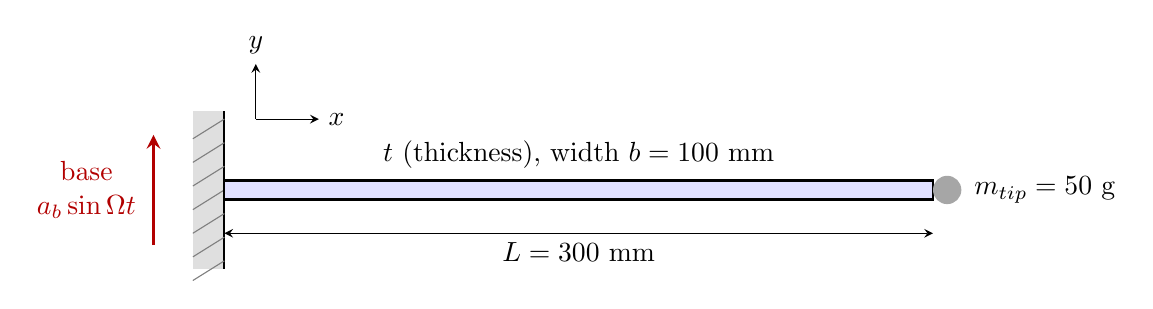
\begin{tikzpicture}[scale=1.0, >=stealth]
  % wall
  \fill[gray!25] (-0.4,-1.0) rectangle (0,1.0);
  \draw[thick] (0,-1.0) -- (0,1.0);
  \foreach \y in {-0.9,-0.6,...,0.9} \draw[gray] (-0.4,\y-0.25) -- (0,\y);
  % plate (side view)
  \fill[blue!12] (0,-0.12) rectangle (9,0.12);
  \draw[thick] (0,-0.12) rectangle (9,0.12);
  % tip mass
  \fill[gray!70] (9.18,0) circle (0.18);
  \node[right] at (9.4,0) {$m_{tip}=50$~g};
  % base excitation
  \draw[->, very thick, red!70!black] (-0.9,-0.7) -- (-0.9,0.7);
  \node[left, align=center, red!70!black] at (-1.0,0) {base\\$a_b\sin\Omega t$};
  % dimensions
  \draw[<->] (0,-0.55) -- (9,-0.55);
  \node[below] at (4.5,-0.55) {$L = 300$ mm};
  \node[above] at (4.5,0.15) {$t$ (thickness), width $b=100$ mm};
  % axes
  \draw[->] (0.4,0.9) -- (1.2,0.9) node[right] {$x$};
  \draw[->] (0.4,0.9) -- (0.4,1.6) node[above] {$y$};
\end{tikzpicture}
\caption{Simplified panel model: cantilever plate clamped at the hinge, with a tip
mass and base excitation in the thickness direction.}
\label{fig:sketch}
\end{figure}

The following assumptions were made:
\begin{itemize}[nosep,leftmargin=2.5em]
  \item The hinge is rigid (clamped boundary). A real hinge is flexible, so this
        assumption gives a frequency that is too high. This is the reason for the
        design margin below.
  \item The tip mass is a point mass without rotary inertia.
  \item Material behavior is linear elastic and damping is viscous with a constant
        modal damping ratio $\zeta = 0.02$ ($Q = 25$), which is inside the range
        given in the user's guide~\cite{rideshare}.
  \item In reality the panel is folded and held at several points during launch. The
        cantilever case is the softest configuration and therefore conservative.
\end{itemize}

\subsection{Requirement and Design Target}

The requirement is $f_1 \geq 40$~Hz~\cite{rideshare}. Since the finite element
models are idealized (rigid hinge, ideal material), a 10\% margin was added, so the
design target is $f_1 \geq 44$~Hz. Two materials were considered; their properties
are listed in Table~\ref{tab:mat}.

\begin{table}[H]
\centering
\caption{Material properties used in the analysis}
\label{tab:mat}
\begin{tabular}{lcccc}
\toprule
Material & $E$, GPa & $\rho$, kg/m$^3$ & $\nu$ & Strength, MPa \\
\midrule
Aluminum 6061-T6~\cite{asm} & 68.9 & 2700 & 0.33 & 276 (yield) \\
Quasi-isotropic CFRP (typical) & 50.0 & 1550 & 0.30 & $\approx$400 \\
\bottomrule
\end{tabular}
\end{table}

\noindent The CFRP properties are typical values for a quasi-isotropic carbon/epoxy
laminate and depend strongly on the layup. They are used only for the concept comparison.

% ---------------------------------------------------------------------
\section{Theory}

\subsection{Natural Frequencies of a Cantilever}

For a uniform Euler--Bernoulli cantilever without tip mass, the natural frequencies
are~\cite{blevins,rao}
\begin{equation}
  \omega_i = (\beta_i L)^2 \sqrt{\frac{EI}{\rho A L^4}}, \qquad
  \beta_1 L = 1.8751,\;\; \beta_2 L = 4.6941,\;\; \beta_3 L = 7.8548
  \label{eq:exact}
\end{equation}
where $I = b t^3/12$ and $A = bt$. With a tip mass, a good estimate of the first
frequency is obtained by the Rayleigh method, where 33/140 of the beam mass $m_b$ is
added to the tip mass~\cite{blevins}:
\begin{equation}
  f_1 \approx \frac{1}{2\pi}\sqrt{\frac{3EI}{L^3\,(m_{tip} + 0.2357\,m_b)}}
  \label{eq:rayleigh}
\end{equation}

\subsection{Beam Finite Element Model}

To get more than one mode and to compute the forced response, the cantilever was
divided into $n$ two-node Euler--Bernoulli beam elements with two degrees of freedom
per node (deflection $w$ and rotation $\theta$). The element stiffness and
consistent mass matrices are~\cite{logan}
\begin{equation}
\mathbf{k}_e = \frac{EI}{L_e^3}
\begin{bmatrix}
 12 & 6L_e & -12 & 6L_e \\
 6L_e & 4L_e^2 & -6L_e & 2L_e^2 \\
 -12 & -6L_e & 12 & -6L_e \\
 6L_e & 2L_e^2 & -6L_e & 4L_e^2
\end{bmatrix},
\qquad
\mathbf{m}_e = \frac{\rho A L_e}{420}
\begin{bmatrix}
 156 & 22L_e & 54 & -13L_e \\
 22L_e & 4L_e^2 & 13L_e & -3L_e^2 \\
 54 & 13L_e & 156 & -22L_e \\
 -13L_e & -3L_e^2 & -22L_e & 4L_e^2
\end{bmatrix}
\end{equation}
After assembly, the tip mass is added to the deflection degree of freedom of the last
node, and the two degrees of freedom of the clamped node are removed. The natural
frequencies and mode shapes follow from the generalized eigenvalue problem
\begin{equation}
  \left(\mathbf{K} - \omega^2 \mathbf{M}\right)\boldsymbol{\phi} = \mathbf{0}
\end{equation}

\subsection{Response to Base Excitation}

When the clamp moves with acceleration $a_b \sin\Omega t$, the motion $\mathbf{u}$
relative to the base satisfies
\begin{equation}
  \mathbf{M}\ddot{\mathbf{u}} + \mathbf{C}\dot{\mathbf{u}} + \mathbf{K}\mathbf{u}
  = -\mathbf{M}\mathbf{r}\,a_b \sin\Omega t
\end{equation}
where $\mathbf{r}$ has ones at the deflection degrees of freedom and zeros at the
rotations. Using mass-normalized modes $\boldsymbol{\phi}_j$ and modal damping, each
mode responds independently with the complex amplitude~\cite{rao,ecss}
\begin{equation}
  q_j = \frac{-\Gamma_j\, a_b}{\omega_j^2 - \Omega^2 + 2i\zeta\omega_j\Omega},
  \qquad \Gamma_j = \boldsymbol{\phi}_j^T \mathbf{M}\mathbf{r}
\end{equation}
The value $\Gamma_j^2$ is the effective modal mass, i.e.\ the part of the mass that
moves with mode $j$ when the base is shaken. The absolute tip acceleration is
$a_b - \Omega^2 u_{tip}$, and the bending stress at the root is
$\sigma = E\,\kappa\,t/2$, where $\kappa$ is the curvature at the clamp.

\subsection{Sandwich Panel}

For a sandwich panel with two face sheets of thickness $t_f$ and a core of thickness
$h_c$, the bending stiffness is carried almost only by the faces. With the distance
between face mid-planes $d = h_c + t_f$, the bending stiffness is~\cite{zenkert}
\begin{equation}
  EI \approx \frac{E_f\, b\, t_f\, d^2}{2}
\end{equation}
Core shear deformation was neglected, which makes the predicted frequency slightly
too high.

% ---------------------------------------------------------------------
\section{MATLAB Model and Verification}

The equations above were programmed in MATLAB. Before using the code for design,
it was tested on a bare aluminum cantilever ($t = 2$~mm, no tip mass), for which
Eq.~(\ref{eq:exact}) gives the exact answer: $f_1 = 18.13$~Hz, $f_2 = 113.64$~Hz and
$f_3 = 318.21$~Hz. Table~\ref{tab:conv} and \figref{fig:conv} show that the error
decreases quickly with the number of elements. With 8 elements the first frequency
is already within 0.001\% of the exact value. All later calculations used 40 elements.

\begin{table}[H]
\centering
\caption{Convergence of the MATLAB beam model (bare cantilever, $t = 2$~mm)}
\label{tab:conv}
\begin{tabular}{ccccccc}
\toprule
Elements & $f_1$, Hz & Error, \% & $f_2$, Hz & Error, \% & $f_3$, Hz & Error, \% \\
\midrule
2  & 18.143 & 0.048  & 114.61 & 0.85   & 387.63 & 21.8 \\
4  & 18.135 & 0.003  & 113.78 & 0.12   & 320.67 & 0.77 \\
8  & 18.134 & $<$0.001 & 113.65 & 0.008 & 318.40 & 0.061 \\
16 & 18.134 & $<$0.001 & 113.65 & $<$0.001 & 318.22 & 0.004 \\
\midrule
Exact & 18.134 & -- & 113.64 & -- & 318.21 & -- \\
\bottomrule
\end{tabular}
\end{table}

\begin{figure}[htbp]
\centering
\begin{subfigure}{0.49\linewidth}
  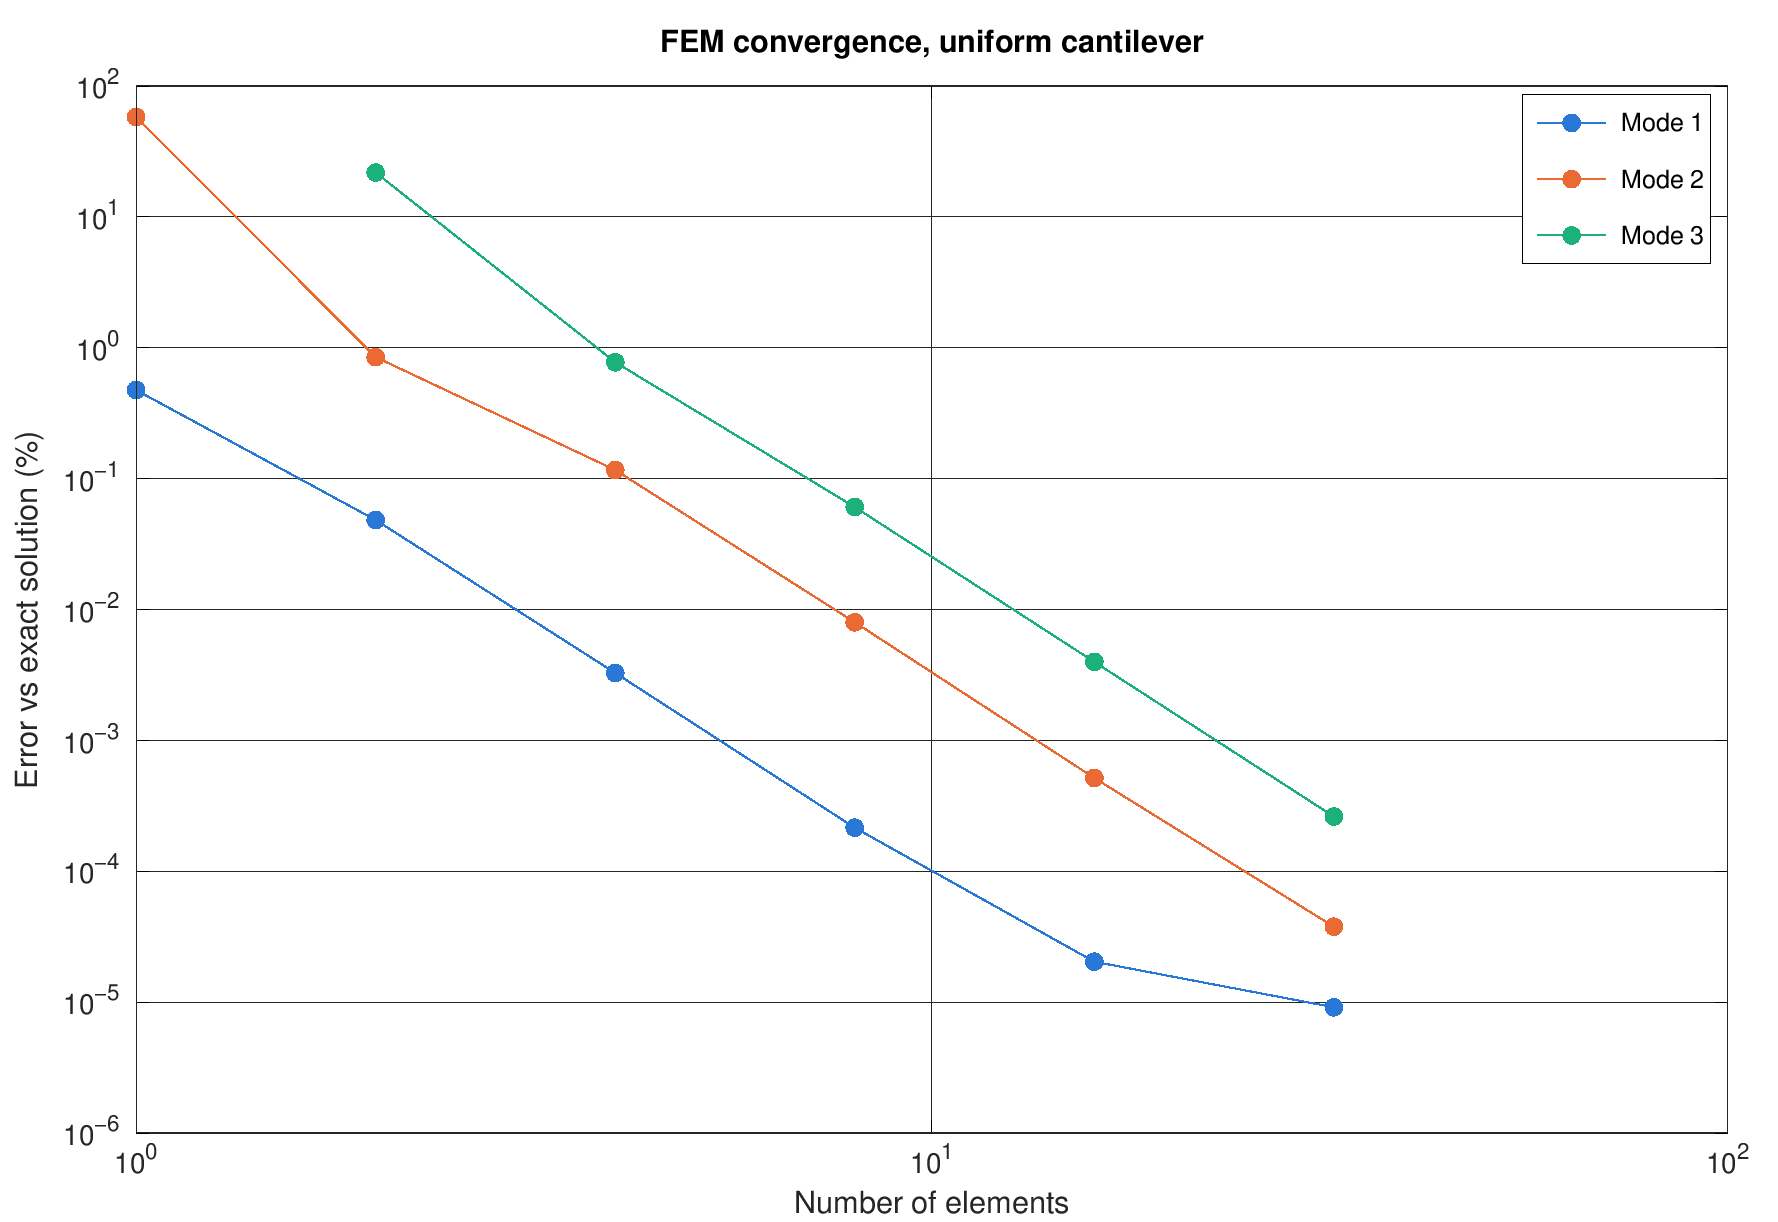
\includegraphics[width=\linewidth]{fig1_convergence.png}
  \caption{Error versus number of elements}
  \label{fig:conv}
\end{subfigure}
\hfill
\begin{subfigure}{0.49\linewidth}
  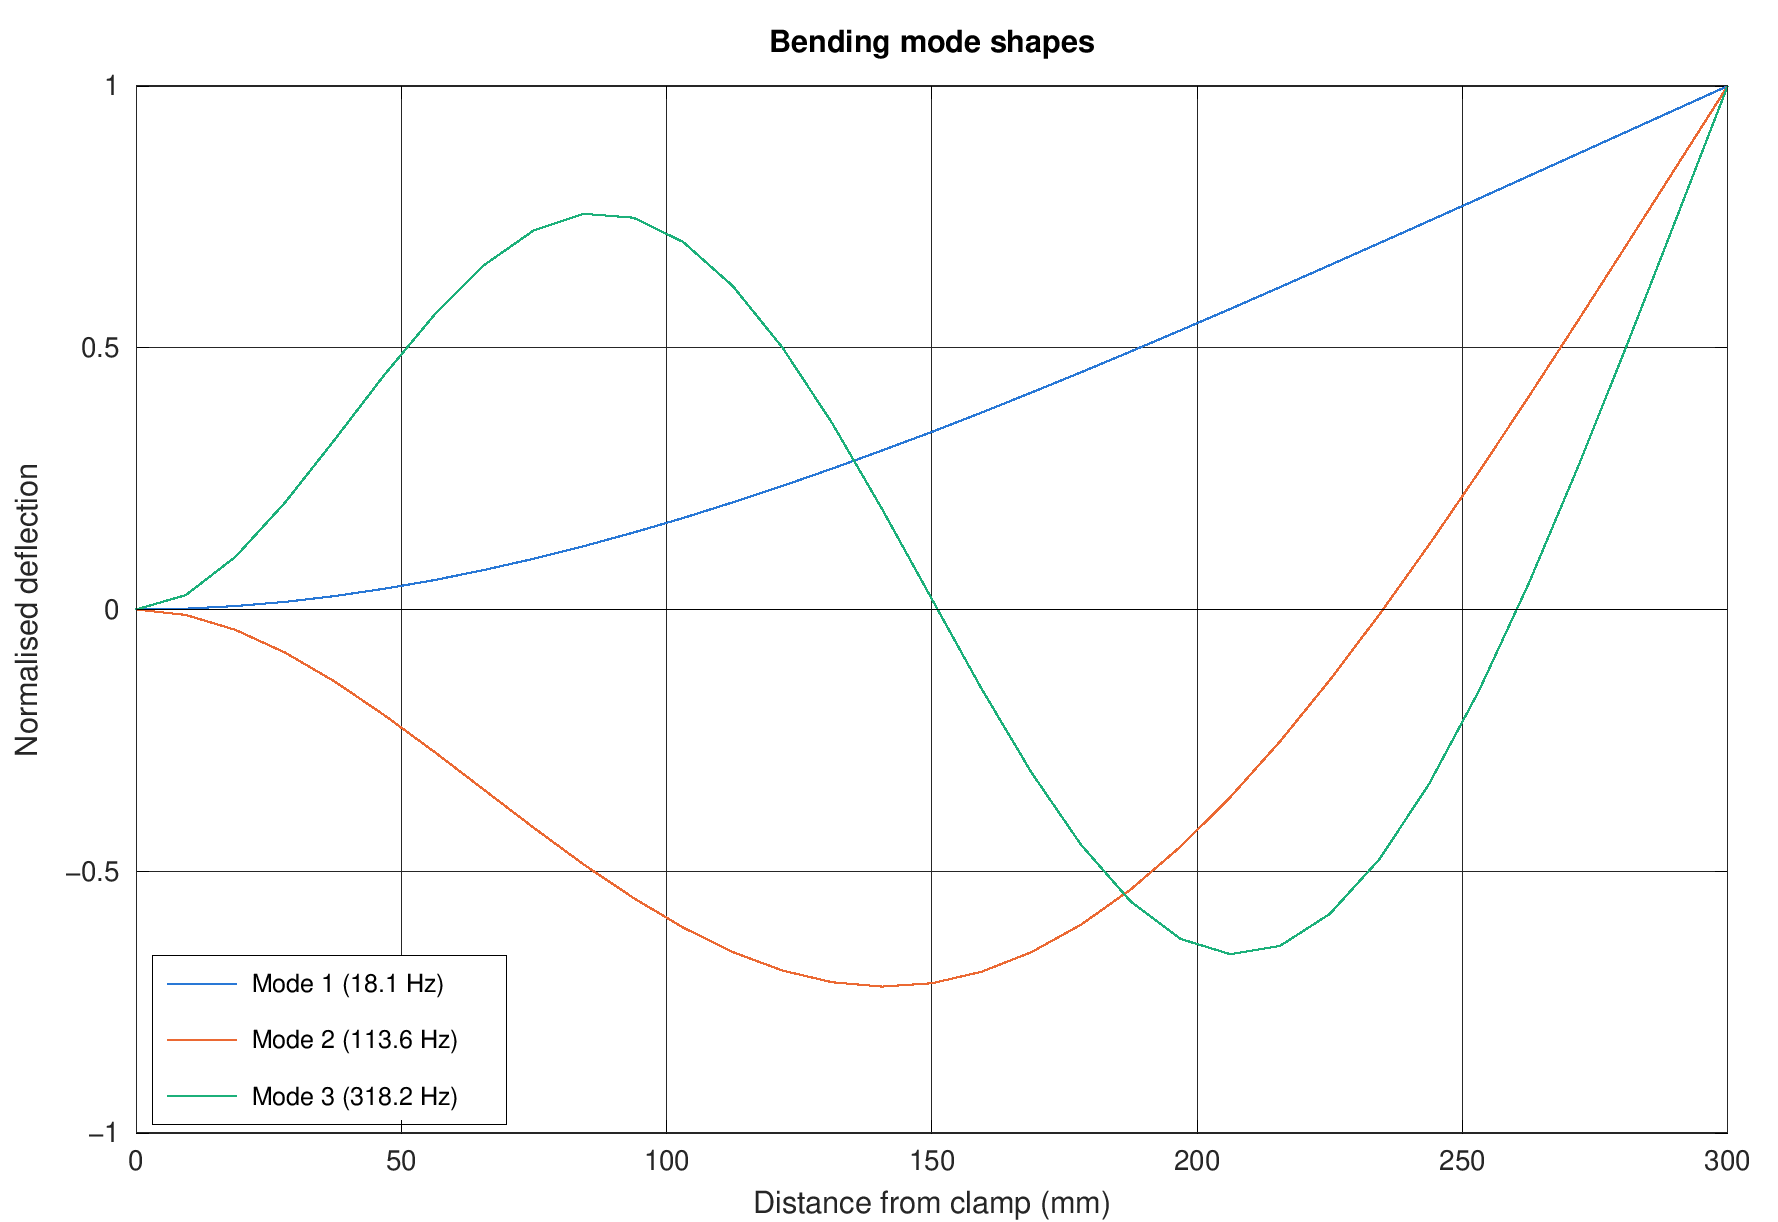
\includegraphics[width=\linewidth]{fig2_mode_shapes.png}
  \caption{First three bending mode shapes}
  \label{fig:shapes}
\end{subfigure}
\caption{Verification of the MATLAB beam model on a uniform cantilever.}
\end{figure}

% ---------------------------------------------------------------------
\section{Design Study}

\subsection{Solid Panels}

The first natural frequency was computed for thicknesses from 1 to 6~mm, using
commercially available sheet thicknesses. Table~\ref{tab:design} shows the aluminum
results together with the hand estimate from Eq.~(\ref{eq:rayleigh}). The two methods
agree within 1\%, so both can be trusted. The bending stiffness grows with $t^3$,
while the panel mass grows only with $t$, so $f_1$ grows a little faster than
linearly with $t$. For a solid plate of a given material, the only way to raise the
frequency is to make it thicker, and each extra millimeter of aluminum adds 81~g.
The thinnest aluminum sheet that meets the 44~Hz target is 6~mm thick, with
$f_1 = 45.7$~Hz and a mass of 486~g (\figref{fig:thick}).

\begin{table}[H]
\centering
\caption{First natural frequency of the solid aluminum panel with 50 g tip mass}
\label{tab:design}
\begin{tabular}{ccccc}
\toprule
$t$, mm & $f_1$ FEM, Hz & $f_1$ Eq.~(\ref{eq:rayleigh}), Hz & Panel mass, g & $f_1 \geq 44$ Hz? \\
\midrule
2.0 & 12.07 & 12.11 & 162 & no \\
3.0 & 20.08 & 20.17 & 243 & no \\
4.0 & 28.46 & 28.61 & 324 & no \\
5.0 & 37.03 & 37.27 & 405 & no \\
6.0 & \textbf{45.73} & 46.06 & 486 & \textbf{yes} \\
\bottomrule
\end{tabular}
\end{table}

A solid CFRP panel behaves in a similar way. It needs the same 6~mm thickness
($f_1 = 46.6$~Hz) but weighs 279~g, because carbon fiber has a higher
stiffness-to-density ratio than aluminum. Even so, both solid panels are heavy for
a small satellite.

\subsection{Honeycomb Sandwich Panel}

Real solar panels are not solid plates but sandwich panels. In a second design
iteration, a panel with two 0.3~mm aluminum face sheets and an aluminum honeycomb core
(density 50~kg/m$^3$) was analyzed. An 8~mm core gives $f_1 = 55.3$~Hz at a panel mass of
only 65~g, including an assumed adhesive mass of 0.15~kg/m$^2$. Compared with the 6~mm
solid aluminum panel, this is an 87\% mass reduction while the frequency is 21\%
higher. \figref{fig:concepts} shows why. For the sandwich, a small increase in mass
gives a large increase in frequency, because the stiffness grows with the square of
the core thickness, and the core itself is very light.

\begin{figure}[htbp]
\centering
\begin{subfigure}{0.49\linewidth}
  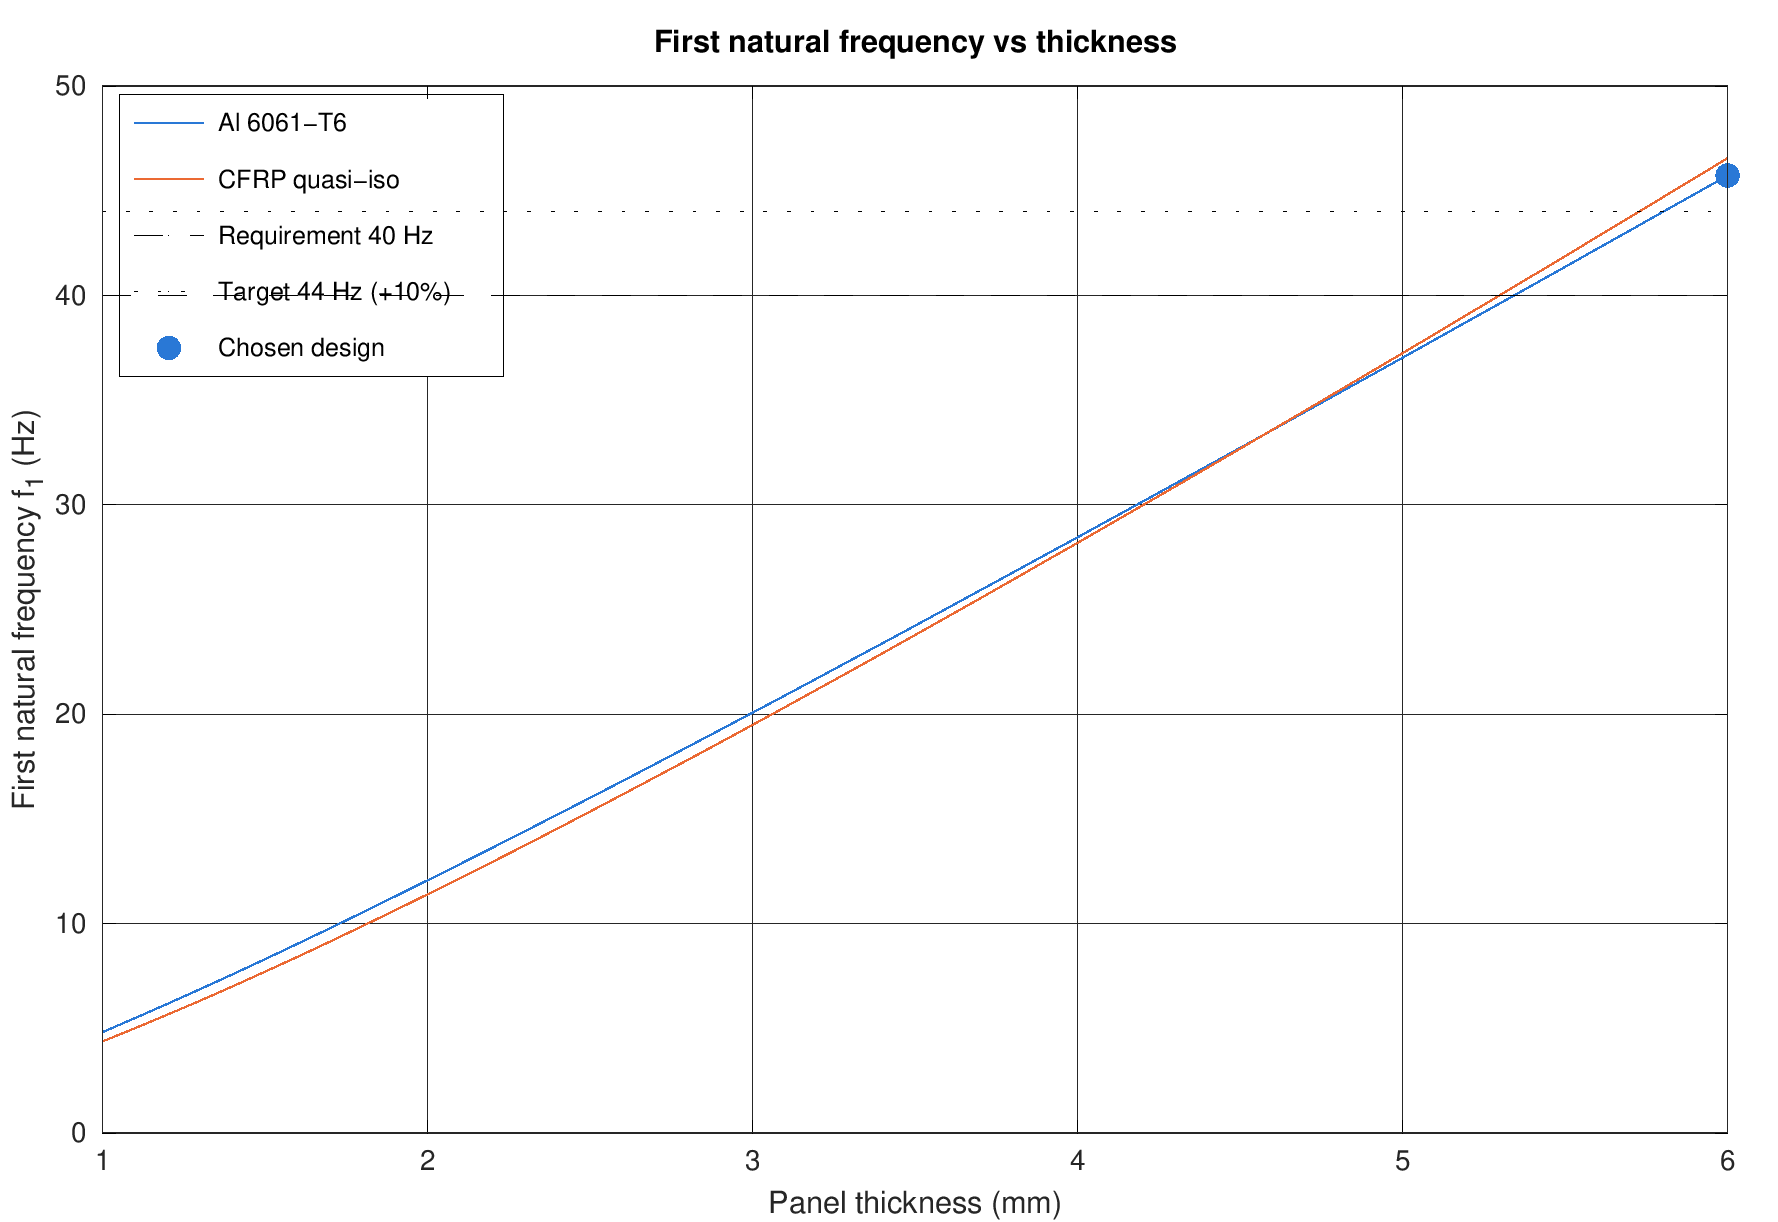
\includegraphics[width=\linewidth]{fig3_f1_vs_thickness.png}
  \caption{$f_1$ versus thickness, solid panels}
  \label{fig:thick}
\end{subfigure}
\hfill
\begin{subfigure}{0.49\linewidth}
  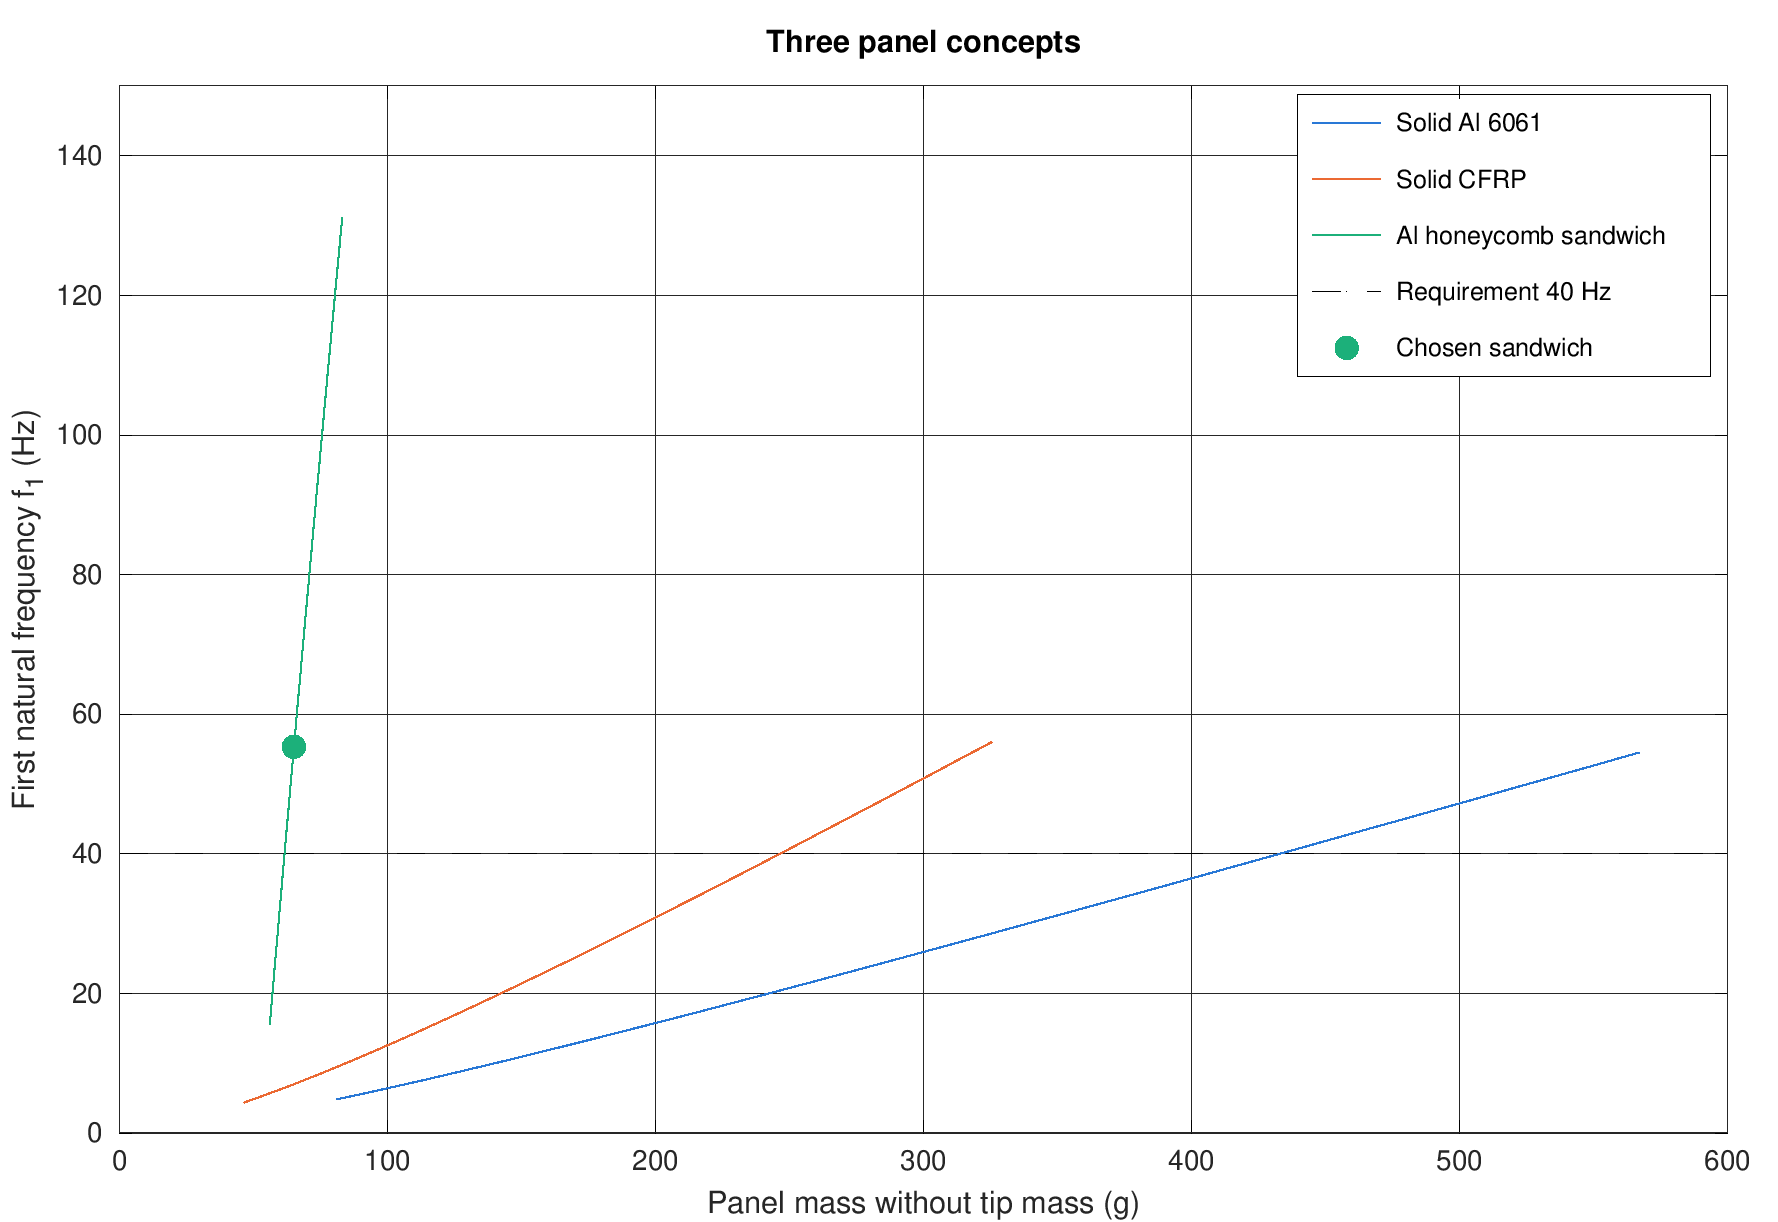
\includegraphics[width=\linewidth]{fig7_concepts.png}
  \caption{$f_1$ versus panel mass, three concepts}
  \label{fig:concepts}
\end{subfigure}
\caption{Design study results. The dashed line is the 40 Hz requirement.}
\end{figure}

For the ANSYS verification the 6~mm solid aluminum panel was chosen, because it is
isotropic, easy to model and can be compared directly with the beam model. The
sandwich panel is the recommended design, and its verification in ANSYS is left for
future work.

% ---------------------------------------------------------------------
\section{ANSYS Finite Element Model}

\subsection{Model Setup}

The panel geometry ($300 \times 100 \times 6$~mm) was created in SolidWorks and
imported into ANSYS Mechanical 2026 R1 (Student). A custom material with the
aluminum properties of Table~\ref{tab:mat} was defined, because the default ANSYS
aluminum alloy has slightly different values. The panel was meshed with hexahedral
solid elements (\figref{fig:mesh}). The hinge end face was fixed (Fixed Support),
and the 50~g tip mass was applied as a Point Mass on the free end face with
deformable behavior, so that it acts at the center of that face.

\begin{figure}[htbp]
\centering
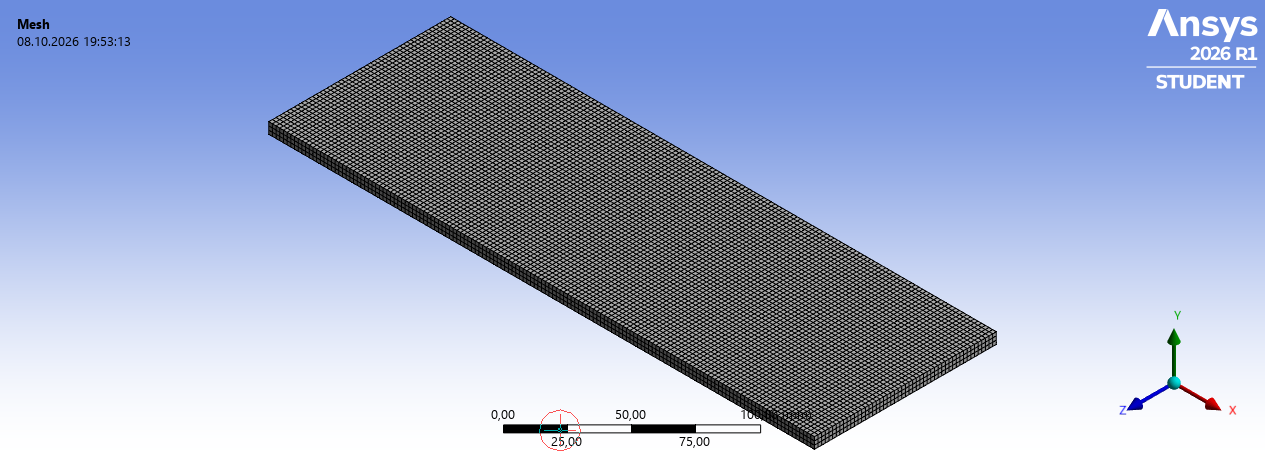
\includegraphics[width=0.55\linewidth, trim=200 20 220 0, clip]{mesh.png}
\caption{ANSYS mesh with 2 mm element size (three elements through the thickness).}
\label{fig:mesh}
\end{figure}

\subsection{Mesh Convergence}

The modal analysis was repeated with element sizes of 10, 5, 3 and 2~mm
(Table~\ref{tab:ansysconv}, \figref{fig:ansysconv}). Refining from 3 to 2~mm changes
the first frequency by only 0.02\%, and all six frequencies change by less than 0.03\%.
The mesh is therefore converged. The 3~mm mesh was used for the harmonic analysis.

\begin{table}[H]
\centering
\caption{ANSYS natural frequencies (Hz) for different element sizes}
\label{tab:ansysconv}
\begin{tabular}{ccccccc}
\toprule
Element size & Mode 1 & Mode 2 & Mode 3 & Mode 4 & Mode 5 & Mode 6 \\
\midrule
10 mm & 46.885 & 305.10 & 333.81 & 715.86 & 876.71 & 1049.2 \\
5 mm  & 46.782 & 304.39 & 333.38 & 715.66 & 874.63 & 1047.7 \\
3 mm  & 46.707 & 303.85 & 332.55 & 715.54 & 872.79 & 1044.9 \\
2 mm  & 46.696 & 303.77 & 332.47 & 715.47 & 872.55 & 1044.7 \\
\bottomrule
\end{tabular}
\end{table}

\begin{figure}[htbp]
\centering
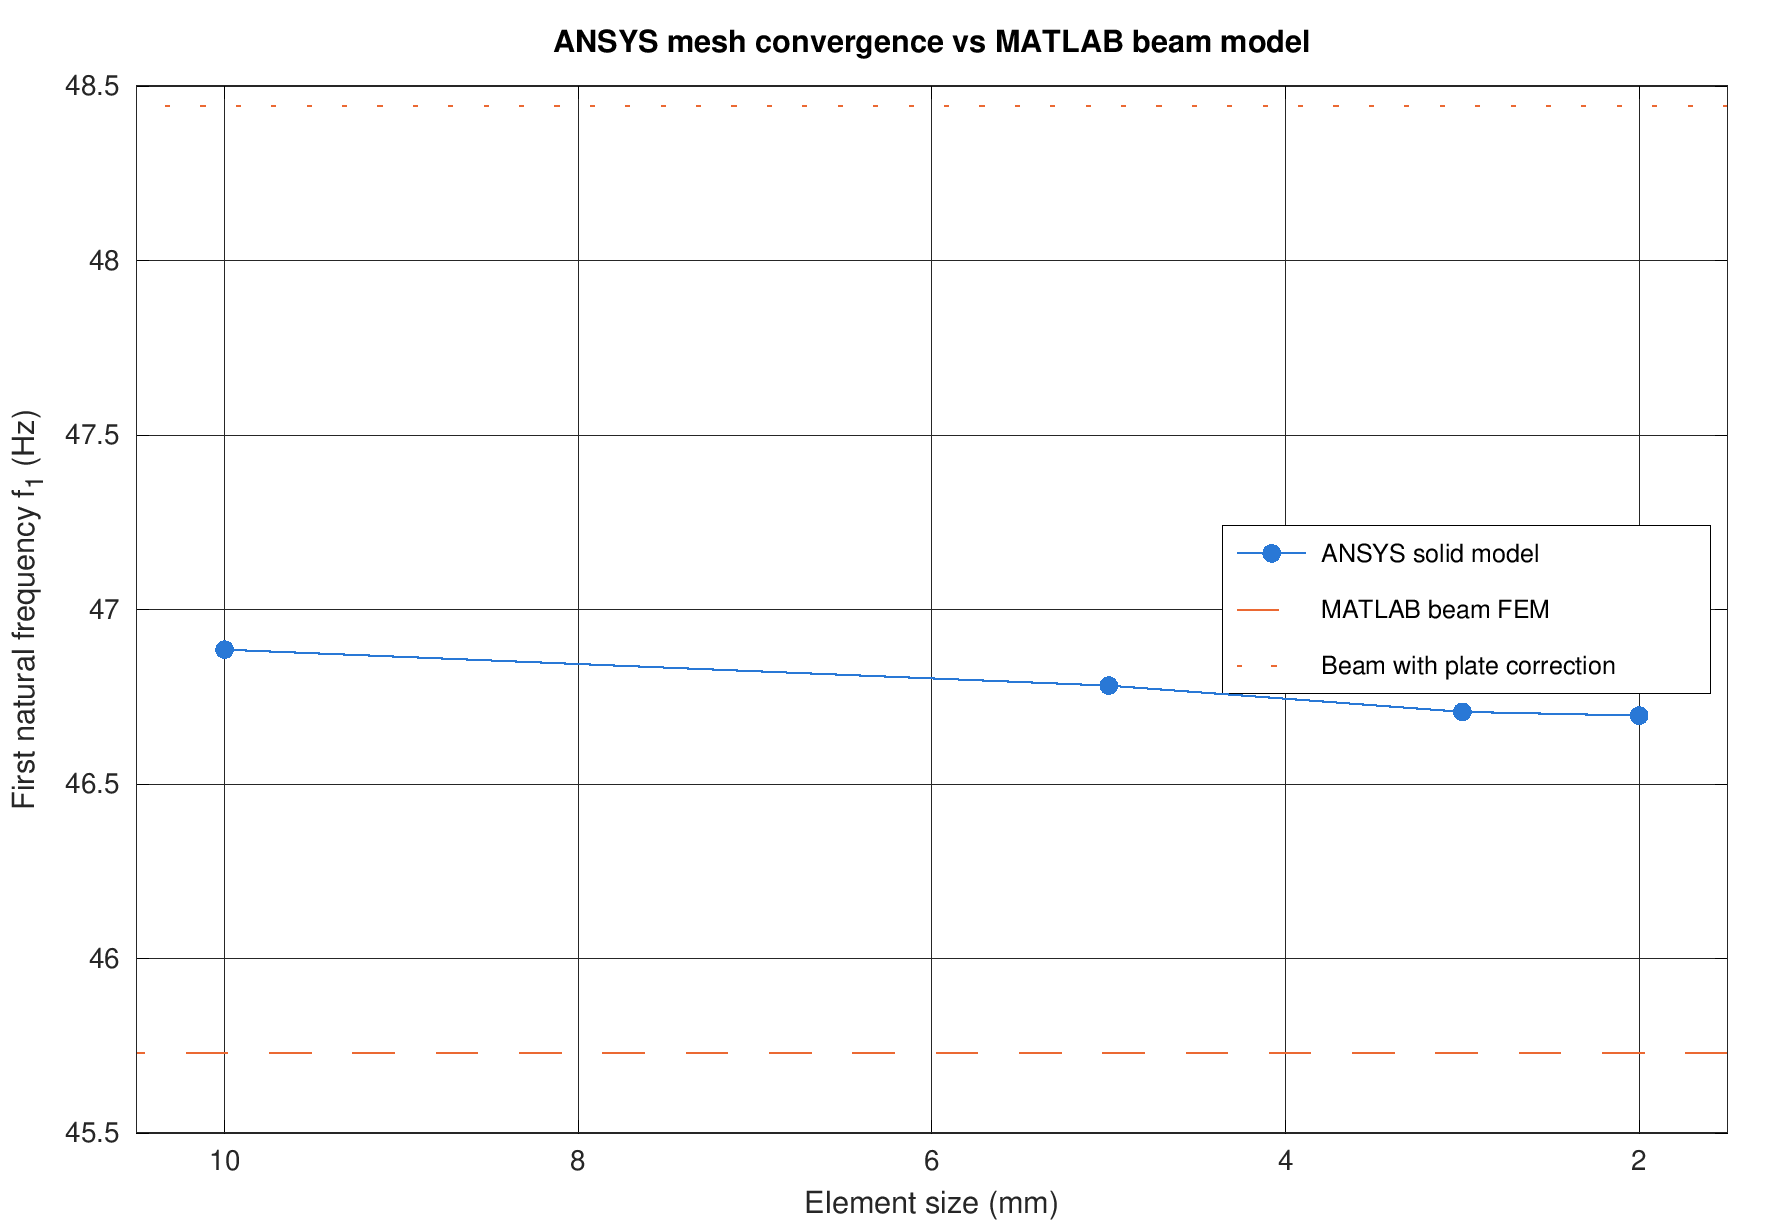
\includegraphics[width=0.6\linewidth]{fig8_ansys_convergence.png}
\caption{Convergence of the ANSYS first natural frequency compared with the MATLAB
beam model and the beam model with plate correction.}
\label{fig:ansysconv}
\end{figure}

\subsection{Mode Shapes and Comparison with MATLAB}

The first four mode shapes are shown in \figref{fig:ansysmodes}. Mode 1 is the first
bending mode in the thickness direction and is the mode that matters for the
requirement. Mode 2 is the second bending mode, mode 3 is the first torsion mode and
mode 4 is bending in the plane of the panel. The beam model cannot predict torsion and
in-plane bending, so only the bending modes can be compared.

\begin{figure}[htbp]
\centering
\begin{subfigure}{0.49\linewidth}
  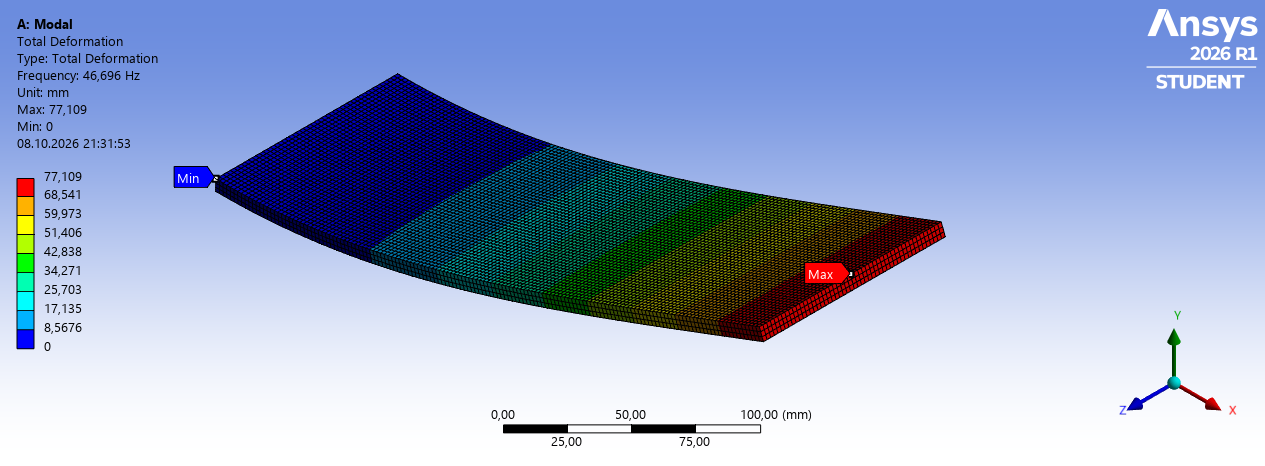
\includegraphics[width=\linewidth, trim=0 0 120 0, clip]{mode1.png}
  \caption{Mode 1: first bending, 46.70 Hz}
\end{subfigure}
\hfill
\begin{subfigure}{0.49\linewidth}
  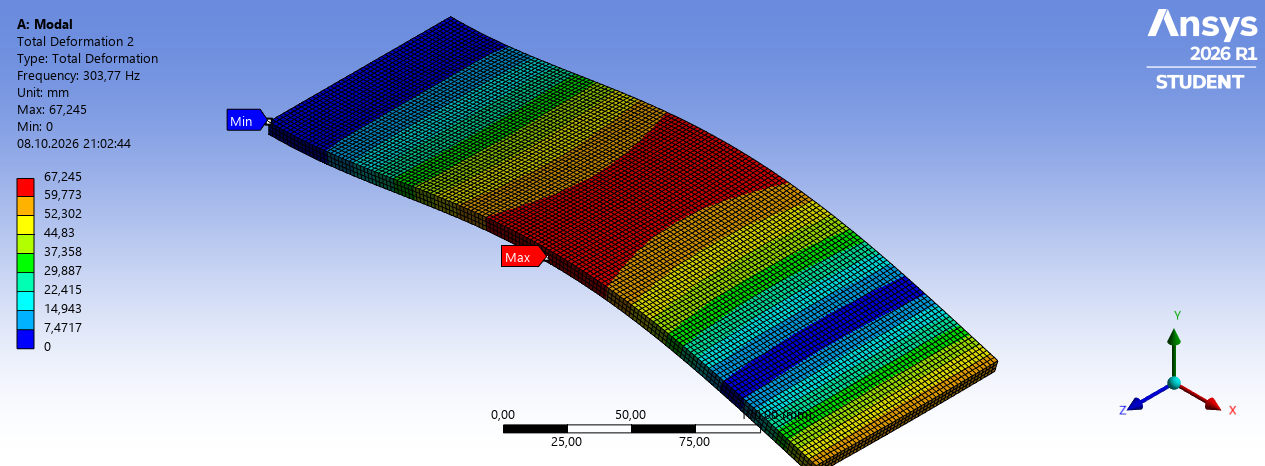
\includegraphics[width=\linewidth, trim=0 0 120 0, clip]{mode2.png}
  \caption{Mode 2: second bending, 303.77 Hz}
\end{subfigure}
\\[6pt]
\begin{subfigure}{0.49\linewidth}
  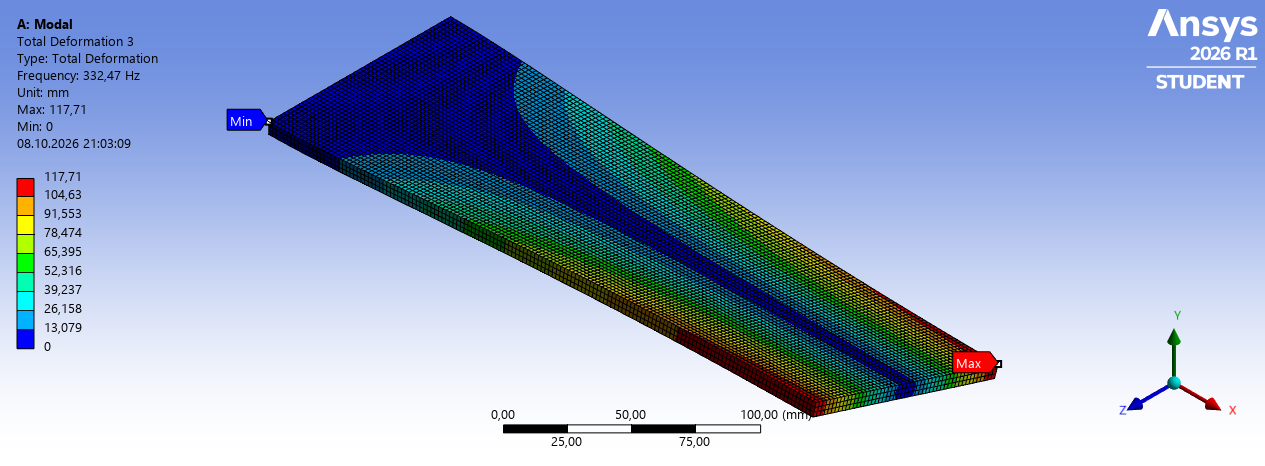
\includegraphics[width=\linewidth, trim=0 0 120 0, clip]{mode3.png}
  \caption{Mode 3: first torsion, 332.47 Hz}
\end{subfigure}
\hfill
\begin{subfigure}{0.49\linewidth}
  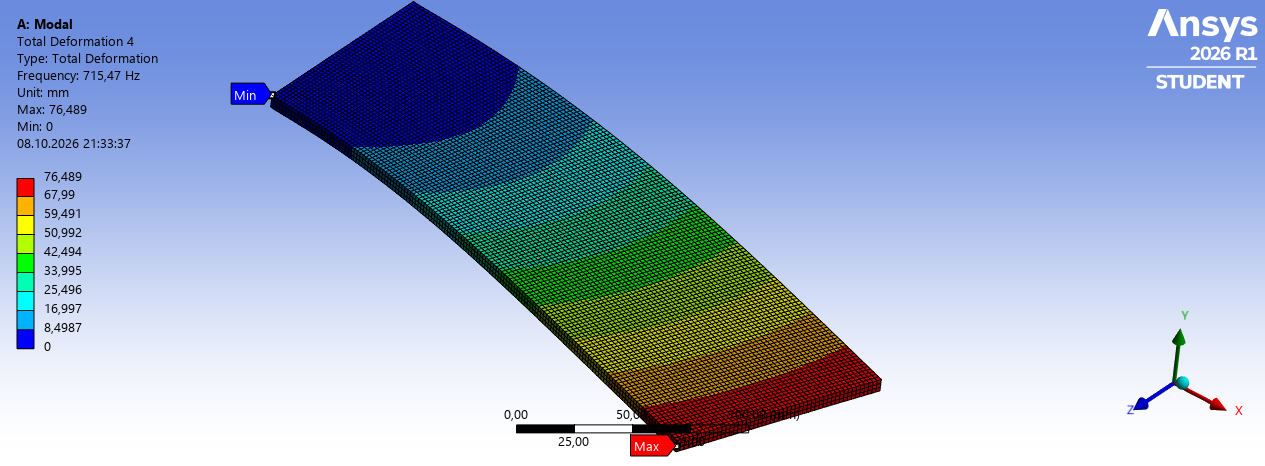
\includegraphics[width=\linewidth, trim=0 0 120 0, clip]{mode4.png}
  \caption{Mode 4: in-plane bending, 715.47 Hz}
\end{subfigure}
\caption{First four mode shapes from ANSYS (2 mm mesh).}
\label{fig:ansysmodes}
\end{figure}

\begin{table}[H]
\centering
\caption{Bending frequencies: ANSYS (2 mm mesh) versus MATLAB beam model}
\label{tab:compare}
\begin{tabular}{lcccc}
\toprule
Mode & ANSYS, Hz & Beam FEM, Hz & Beam with plate correction, Hz & Difference ANSYS--Beam \\
\midrule
1st bending & 46.70  & 45.73  & 48.44  & +2.1\% \\
2nd bending & 303.77 & 298.78 & 316.51 & +1.7\% \\
3rd bending & 872.55 & 857.70 & 908.60 & +1.7\% \\
\bottomrule
\end{tabular}
\end{table}

As seen in Table~\ref{tab:compare}, ANSYS gives frequencies about 2\% higher than the
beam model. The reason is that the panel is a wide plate and not a narrow beam. In a
beam, the cross-section can freely contract and expand sideways (Poisson effect),
while in a wide plate this is partly prevented, which makes the plate stiffer. In
the limit of a very wide plate, $E$ should be replaced by $E/(1-\nu^2)$, which raises
the frequency by $1/\sqrt{1-\nu^2} = 5.9\%$. The ANSYS results lie between the beam
value and this upper limit, as expected for a plate with $b/L = 1/3$.

So the main result is that the ANSYS first frequency of 46.7~Hz meets the 40~Hz
requirement with a margin of 16.7\%.

% ---------------------------------------------------------------------
\section{Sine Vibration Response}

The panel response to sine base excitation in the thickness direction was computed
from 5 to 100~Hz with 2\% damping. The exact sine levels depend on the launch vehicle
and are given in the user's guide~\cite{rideshare}. Since the system is linear, the
analysis was done for a unit input of 1~g, and the results can simply be multiplied by
the real level.

In MATLAB, modal superposition with the first four modes was used. The first mode
carries 63\% of the moving mass as effective modal mass, and the first four modes
together carry 92\%. In ANSYS, a Harmonic Response analysis (mode superposition)
linked to the modal analysis was used, with the acceleration applied as base
excitation at the fixed support, 400 frequency steps and absolute results.

\begin{figure}[htbp]
\centering
\begin{subfigure}{0.48\linewidth}
  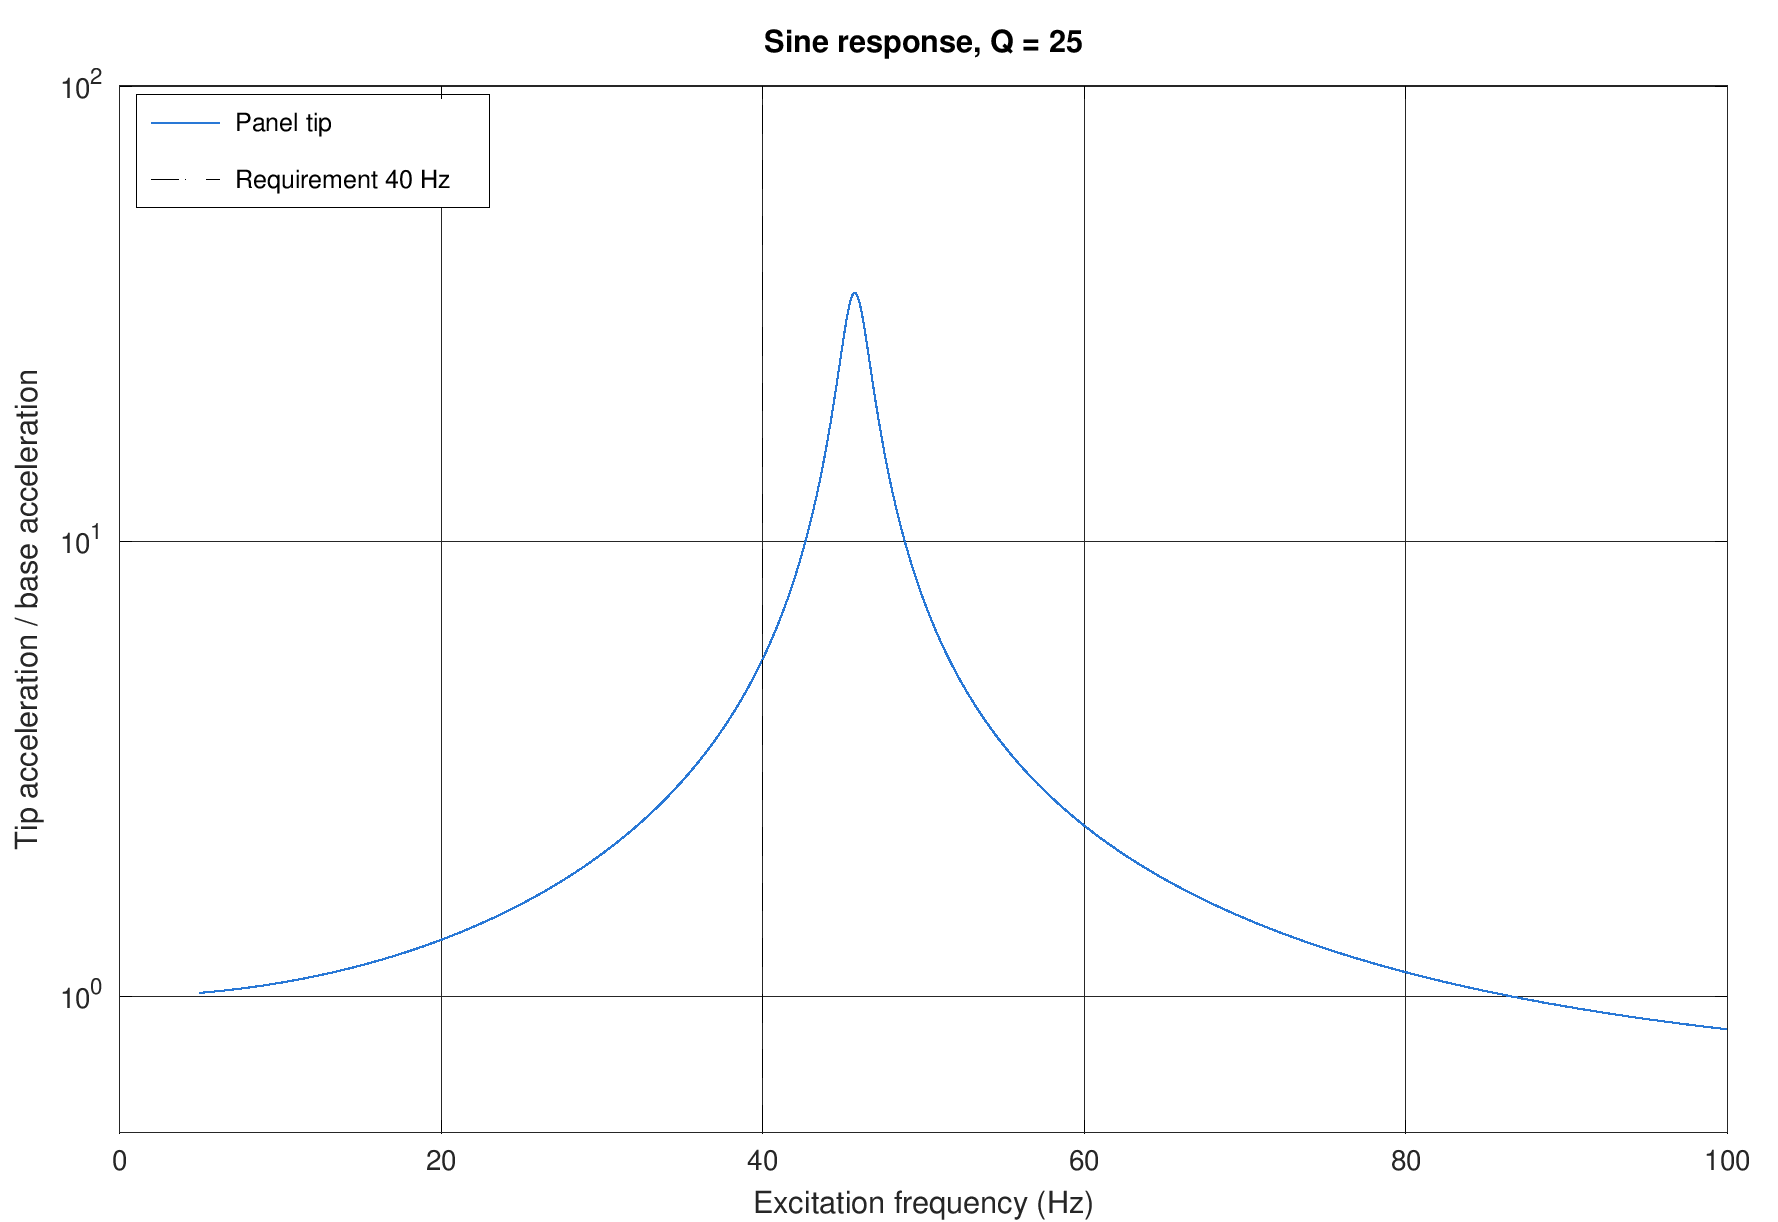
\includegraphics[width=\linewidth]{fig5_transmissibility.png}
  \caption{MATLAB: tip transmissibility}
\end{subfigure}
\hfill
\begin{subfigure}{0.50\linewidth}
  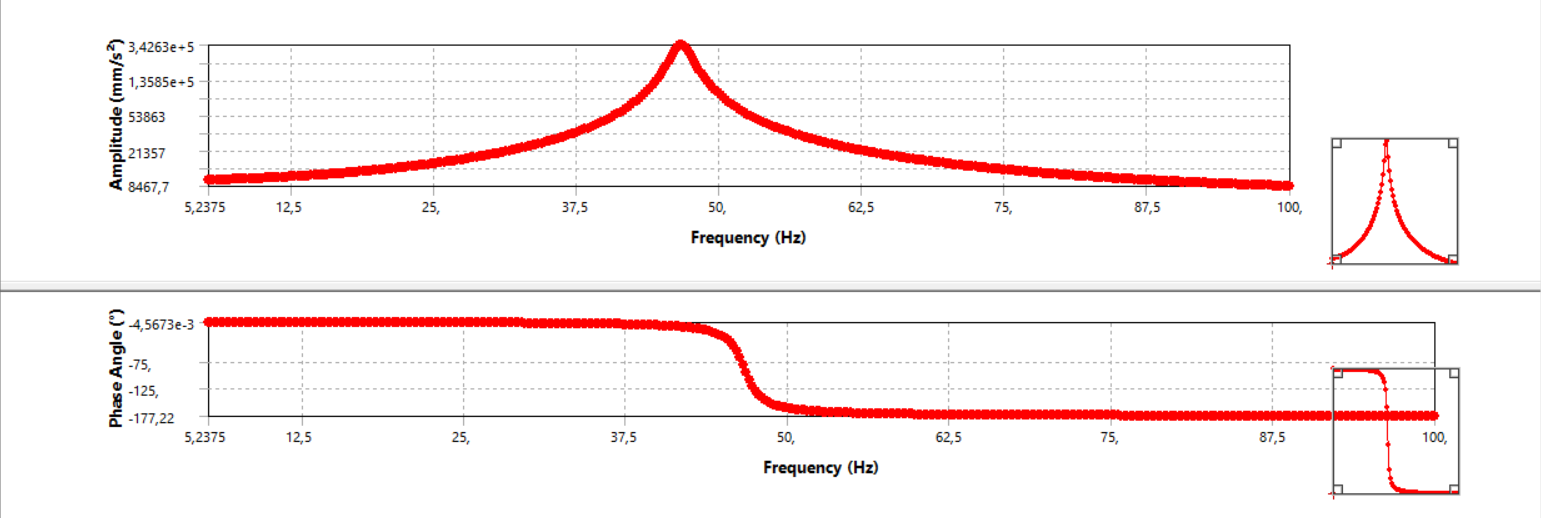
\includegraphics[width=\linewidth, trim=0 0 230 0, clip]{harmonic_tip_acc_crop.png}
  \caption{ANSYS: tip acceleration amplitude (mm/s$^2$) and phase}
\end{subfigure}
\caption{Tip response to 1 g sine base excitation.}
\label{fig:harm}
\end{figure}

\begin{figure}[htbp]
\centering
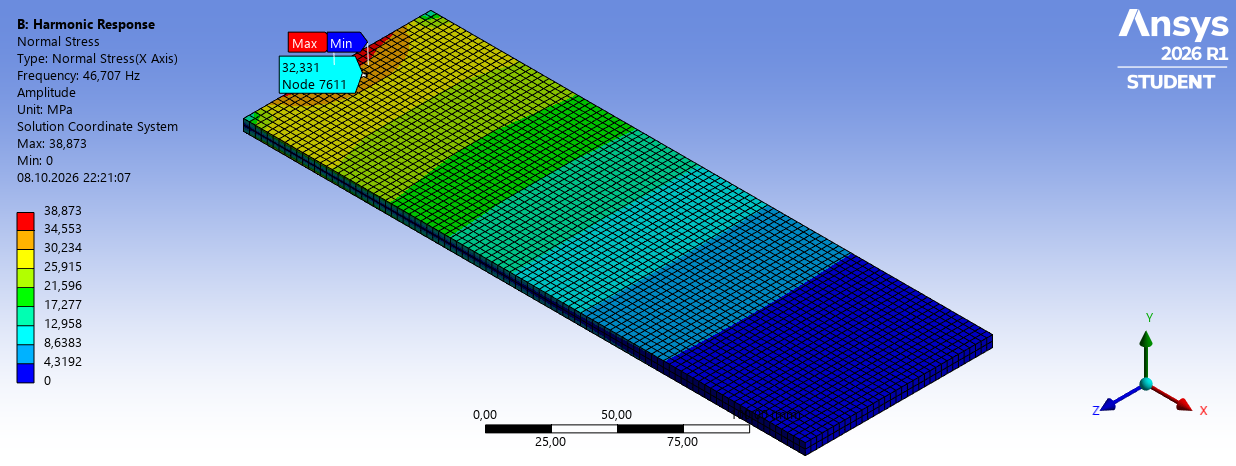
\includegraphics[width=0.75\linewidth, trim=0 0 200 0, clip]{harmonic_stress.png}
\caption{ANSYS normal stress along the panel length at resonance (46.7 Hz, 1 g input).
The probe value of 32.3 MPa is taken at mid-width close to the root.}
\label{fig:stress}
\end{figure}

\begin{table}[H]
\centering
\caption{Sine response at resonance for 1 g base input}
\label{tab:harm}
\begin{tabular}{lccc}
\toprule
Quantity & MATLAB & ANSYS & Difference \\
\midrule
Resonance frequency, Hz & 45.7 & 46.7 & +2.1\% \\
Peak tip acceleration, g & 35.1 & 34.9 & $-0.5$\% \\
Root bending stress, MPa & 32.2 & 32.3 & +0.4\% \\
\bottomrule
\end{tabular}
\end{table}

The results are given in Table~\ref{tab:harm}. The two models agree within 1\% in
amplitude and stress.
At resonance the tip moves about 35 times more strongly than the base. This is larger
than $Q = 25$ because the tip of a cantilever moves more than the average point of the
panel. The phase of the tip response changes from 0$^\circ$ to $-180^\circ$ and passes
$-90^\circ$ at resonance. This is typical when one mode dominates the response. Above
about 85~Hz the tip acceleration becomes smaller than the input, so the panel isolates
higher frequencies.

The maximum stress in ANSYS (38.9~MPa) appears at the corners of the fixed face
(\figref{fig:stress}). This is a stress concentration caused by the perfectly rigid
boundary condition and depends on the mesh, so the probe value at mid-width was used
for comparison. With a factor of safety of 1.25 on yield (a typical value; the
actual factors are set by the launch provider), the margin of safety for 1~g input is
\begin{equation}
  MS = \frac{\sigma_y}{FS \cdot \sigma} - 1 = \frac{276}{1.25 \times 32.3} - 1 = 5.8
\end{equation}
This means that the panel can withstand a sine input of about 6.8~g at resonance
before reaching the allowable stress.

% ---------------------------------------------------------------------
\section{Discussion and Limitations}

The three methods (hand formula, MATLAB beam model and ANSYS solid model) give a
similar results, and the remaining differences have a physical explanation.
Still, the work has some limitations:
\begin{itemize}[nosep,leftmargin=2.5em]
  \item The hinge was modeled as rigid. A real hinge and its bracket add flexibility
        and lower the first frequency, possibly by more than the 16.7\% margin. A test
        or a detailed hinge model is needed.
  \item Damping of 2\% was assumed. Real damping of bolted aluminum structures is
        often between 1\% and 5\%, so the peak response may differ.
  \item The sine levels were normalized to 1~g. The real levels from the user's guide
        must be applied before a final strength check.
  \item The sandwich panel results come only from a simplified beam model without core
        shear deformation, and were not verified in ANSYS.
  \item Only the deployed cantilever configuration was studied. A real panel is stowed
        and held at several hold-down points during launch.
\end{itemize}

% ---------------------------------------------------------------------
\section{Conclusions}

A deployable solar panel of a small satellite was sized against the 40~Hz minimum
frequency requirement of the SpaceX Rideshare Payload User's Guide. The main
conclusions are:
\begin{enumerate}[nosep,leftmargin=2.5em]
  \item A self-written MATLAB beam finite element code reproduced the exact cantilever
        frequencies with less than 0.001\% error and agreed with the Rayleigh estimate
        within 1\%.
  \item A solid aluminum panel needs a thickness of 6~mm to pass the requirement with
        margin, which leads to a heavy panel (486~g).
  \item An aluminum honeycomb sandwich panel with an 8~mm core reaches 55.3~Hz with only
        65~g, an 87\% mass reduction. This explains why real solar panels use sandwich
        construction.
  \item The ANSYS solid model of the 6~mm aluminum panel gives $f_1 = 46.7$~Hz, a 16.7\%
        margin over the requirement, with a converged mesh. It differs from the beam
        model by only 2\%, and the difference is explained by plate effects.
  \item Under 1~g sine base excitation, the peak tip acceleration is about 35~g and the
        root stress is 32.3~MPa. MATLAB and ANSYS agree within 1\%.
\end{enumerate}

Future work should include an ANSYS model of the sandwich panel with core shear, a
model of the hinge stiffness, the real sine and random vibration levels from the
user's guide and, if possible, a simple vibration test to measure the first frequency
and damping.

% ---------------------------------------------------------------------
\section*{Acknowledgments}

The finite element analysis was carried out with ANSYS Mechanical 2026 R1 Student,
the geometry was created in SolidWorks, and the beam model was implemented in MATLAB.

% ---------------------------------------------------------------------
\renewcommand{\refname}{References}
\begin{thebibliography}{9}
\setlength{\itemsep}{0pt}
\small

\bibitem{rideshare}
SpaceX, \textit{Rideshare Payload User's Guide}, Space Exploration Technologies Corp.,
Hawthorne, CA, 2026.

\bibitem{asm}
ASM International, \textit{ASM Handbook, Vol.~2: Properties and Selection:
Nonferrous Alloys and Special-Purpose Materials}, ASM International, Materials Park,
OH, 1990.

\bibitem{blevins}
Blevins, R.~D., \textit{Formulas for Natural Frequency and Mode Shape}, Van Nostrand
Reinhold, New York, 1979.

\bibitem{rao}
Rao, S.~S., \textit{Mechanical Vibrations}, 6th ed., Pearson, Hoboken, NJ, 2017.

\bibitem{logan}
Logan, D.~L., \textit{A First Course in the Finite Element Method}, 6th ed.,
Cengage Learning, Boston, MA, 2017.

\bibitem{ecss}
European Cooperation for Space Standardization, \textit{Spacecraft Mechanical Loads
Analysis Handbook}, ECSS-E-HB-32-26A, ESA Requirements and Standards Division,
Noordwijk, The Netherlands, 2013.

\bibitem{zenkert}
Zenkert, D., \textit{An Introduction to Sandwich Construction}, Engineering Materials
Advisory Services, London, 1995.

\bibitem{wijker}
Wijker, J.~J., \textit{Spacecraft Structures}, Springer, Berlin, 2008.

\end{thebibliography}

\end{document}
